\section{Resultados}\label{cap:resultados}
% orçamento: 2.200 palavras

Este capítulo reúne os resultados quantitativos. Os números das \autoref{sec:res-validacao} e \ref{sec:res-integradores} foram obtidos por uma segunda implementação do núcleo físico, em Python e NumPy, escrita para este relatório a partir do mesmo arquivo de condições iniciais. Ela reproduz, até a última casa decimal publicada, a tabela de validação da documentação do programa. Como usa o mesmo algoritmo e o mesmo passo, confirma o porte para TypeScript, não a física; a física é validada pela comparação com o JPL. Os roteiros estão no \autoref{ap:experimentos}.

\subsection{Validação contra a efeméride do JPL}\label{sec:res-validacao}

Partindo de 1º de janeiro de 2026, o sistema de nove corpos foi integrado para a frente e para trás e comparado com as posições do JPL Horizons nas mesmas datas. O critério de aceitação, fixado \emph{antes} de olhar os resultados, foi erro inferior a 1\,\% da distância ao Sol para todos os corpos no intervalo de $-100$ a $+100$ anos. A comparação foi feita em cinco datas ($-100$, $-10$, $+1$, $+10$ e $+100$ anos), não em varredura contínua. A \autoref{tab:validacao} e a \autoref{fig:validacao} mostram o resultado.

\begin{table}[htb]
  \centering
  \caption{Erro de posição contra o JPL Horizons, em quilômetros}
  \label{tab:validacao}
  \small
  \setlength{\tabcolsep}{4pt}
  \begin{tabular}{lrrrrrrrrr}
    \toprule
    Intervalo & Sol & Mercúrio & Vênus & Terra & Marte & Júpiter & Saturno & Urano & Netuno \\
    \midrule
    $-100$ anos & 153 & 247\,115 & 5\,612 & 4\,782 & 3\,420 & 195 & 173 & 238 & 709 \\
    $-10$ anos  & 4   & 15\,637  & 556    & 489    & 297    & 35  & 8   & 3   & 7 \\
    $+1$ ano    & 0,2 & 3\,048   & 61     & 49     & 35     & 0,4 & 0,1 & 0,0 & 0,1 \\
    $+10$ anos  & 1   & 14\,365  & 534    & 487    & 368    & 41  & 5   & 3   & 7 \\
    $+100$ anos & 112 & 302\,436 & 5\,725 & 4\,763 & 4\,180 & 164 & 142 & 210 & 636 \\
    \bottomrule
  \end{tabular}
  \legend{Integrador de Yoshida de quarta ordem, passo de 0,5 dia, posições relativas ao baricentro do Sistema Solar. Fonte: elaborada pelos autores.}
\end{table}

\begin{figure}[htb]
  \centering
  \caption{Erro relativo à distância ao Sol}
  \label{fig:validacao}
  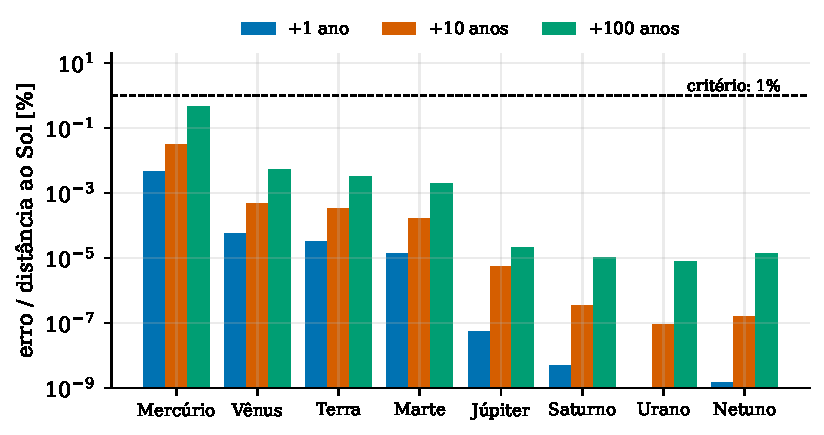
\includegraphics[width=0.95\textwidth]{validacao.pdf}
  \legend{Escala logarítmica. A linha tracejada é o critério de 1\,\%. Fonte: elaborada pelos autores.}
\end{figure}

Todos os corpos passam com folga. O pior caso é Mercúrio: 0,004\,\% da distância ao Sol em um ano, 0,03\,\% em dez e 0,45\,\% em cem. Mercúrio é o caso difícil por duas razões. É o planeta mais rápido, com apenas 176 passos de integração por órbita, e por isso o erro de truncamento do passo pesa mais nele. E é o mais afetado pela relatividade geral, que o modelo não inclui (\autoref{sec:nao-inclui}). Em cem anos, a conservação ficou em $2\times10^{-9}$ para a energia relativa e $1{,}4\times10^{-14}$ para o momento angular.

\subsection{Escolha do integrador}\label{sec:res-integradores}

\subsubsection{Custo e precisão}

A \autoref{fig:trabalho-precisao} compara três integradores pelo critério que importa num programa interativo: quanta precisão se obtém por unidade de custo. O custo é contado em avaliações da força (o \autoref{alg:forca}), que dominam o tempo de execução. A precisão é o erro de Mercúrio após dez anos.

\begin{figure}[htb]
  \centering
  \caption{Precisão em função do custo para três integradores}
  \label{fig:trabalho-precisao}
  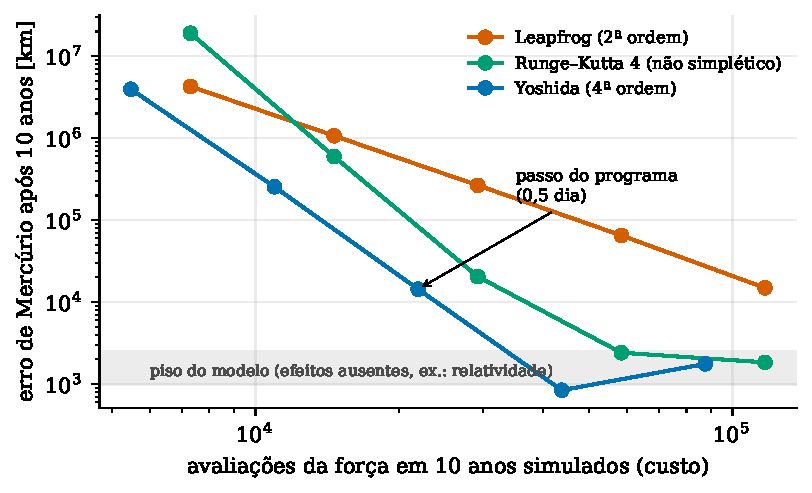
\includegraphics[width=0.9\textwidth]{trabalho_precisao.pdf}
  \legend{Cada ponto é um tamanho de passo. Leapfrog: de 0,5 a 1/32 dia; Yoshida e RK4: de 2 a 0,125 dia. A faixa cinza marca o patamar abaixo do qual o erro não cai, por menor que seja o passo. Fonte: elaborada pelos autores.}
\end{figure}

Do gráfico saem três leituras:

\begin{enumerate}
  \item As inclinações das curvas confirmam as ordens teóricas: reduzir o passo à metade divide o erro do leapfrog por cerca de 4 ($\Delta t^2$) e o do Yoshida por cerca de 16 ($\Delta t^4$), enquanto o passo é grande o bastante para que o truncamento domine.
  \item No passo escolhido, 0,5 dia, o Yoshida gasta 21\,912 avaliações e erra $1{,}4\times10^4$\,km. O leapfrog precisa de mais de 116\,000 avaliações, mais de cinco vezes o custo, para chegar ao mesmo erro.
  \item Abaixo de cerca de $10^3$\,km o erro deixa de cair. Esse patamar não vem do integrador, mas do \emph{modelo}: do que a integração não inclui. Sua ordem de grandeza coincide com a estimativa do efeito relativístico sobre Mercúrio em dez anos feita na \autoref{sec:nao-inclui}. Diminuir o passo além desse ponto só gasta tempo.
\end{enumerate}

\subsubsection{Conservação de energia a longo prazo}

A \autoref{fig:energia} integra o sistema por mil anos com passo deliberadamente grande, de 2 dias, para tornar visível o comportamento qualitativo. O RK4, que não é simplético, apresenta deriva sistemática: ao fim, a energia relativa mudou $4\times10^{-4}$, e a tendência continua. Os dois métodos simpléticos oscilam numa faixa fixa, de $10^{-5}$ para o leapfrog e $3\times10^{-7}$ para o Yoshida, sem tendência. Essa propriedade pesou mais na escolha que a precisão de um passo isolado: um programa que pode ficar rodando por séculos simulados não pode ter órbitas que encolhem ou se expandem aos poucos.

\begin{figure}[htb]
  \centering
  \caption{Erro relativo de energia em mil anos, com passo de 2 dias}
  \label{fig:energia}
  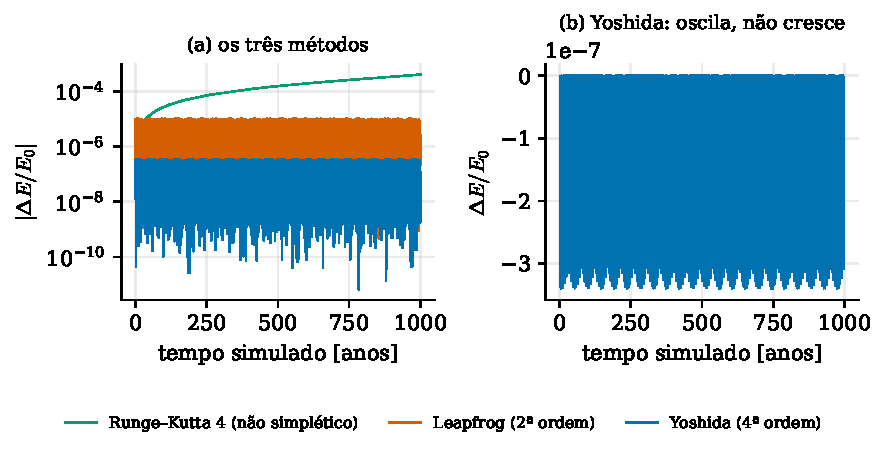
\includegraphics[width=\textwidth]{energia.pdf}
  \legend{(a) Valor absoluto do erro, em escala logarítmica: o RK4 cresce, os simpléticos não. (b) O erro do Yoshida em escala linear: uma oscilação rápida dentro de uma faixa fixa. Fonte: elaborada pelos autores.}
\end{figure}

\begin{noprograma}
Em ``Mostrar dados técnicos'', o programa exibe ao vivo o desvio de energia e de momento angular desde o início da simulação. Deixando o tempo correr por séculos, vê-se o número oscilar sem crescer, o que mostra na prática o significado da palavra simplético.
\end{noprograma}

\subsection{Séries de Fourier das órbitas}\label{sec:res-fourier}

\subsubsection{Convergência}

A \autoref{tab:fourier} e a \autoref{fig:convergencia} mostram, para a elipse osculadora de cada planeta em 1/1/2026, o desvio médio entre a série truncada em $|n|\leq N$ e a órbita. O número de harmônicos necessário cresce com a excentricidade: Vênus, quase circular, chega ao piso de arredondamento ($10^{-12}$\,UA, cerca de 15\,cm) com 6 harmônicos; Mercúrio precisa de 18.

\begin{table}[htb]
  \centering
  \caption{Desvio médio da série truncada em relação à órbita de Kepler}
  \label{tab:fourier}
  \small
  \begin{tabular}{lcrrrc}
    \toprule
    Planeta & $e$ & $|n|\leq1$ (km) & $|n|\leq2$ (km) & $|n|\leq3$ (km) & $N$ até $10^{-12}$\,UA \\
    \midrule
    Mercúrio & 0,2056 & 5\,800\,825  & 887\,349   & 160\,766 & 18 \\
    Vênus    & 0,0068 & 366\,870    & 1\,866     & 11       & 6 \\
    Terra    & 0,0167 & 1\,246\,726 & 15\,587    & 231      & 7 \\
    Marte    & 0,0935 & 10\,597\,766 & 741\,792  & 61\,528  & 12 \\
    Júpiter  & 0,0483 & 18\,756\,268 & 678\,692  & 29\,105  & 10 \\
    Saturno  & 0,0554 & 39\,450\,189 & 1\,636\,812 & 80\,485 & 11 \\
    Urano    & 0,0468 & 67\,447\,711 & 2\,367\,664 & 98\,502 & 10 \\
    Netuno   & 0,0111 & 25\,028\,289 & 208\,577  & 2\,060   & 7 \\
    \bottomrule
  \end{tabular}
  \legend{Elementos osculadores heliocêntricos em 1/1/2026, 720 amostras no tempo. Com $|n|\leq1$ a série tem três termos ($c_{-1}$, $c_0$, $c_1$); falta o epiciclo $c_2\approx\frac12 ae$, que domina o desvio. Fonte: elaborada pelos autores.}
\end{table}

\begin{figure}[htb]
  \centering
  \caption{Convergência da série de Fourier}
  \label{fig:convergencia}
  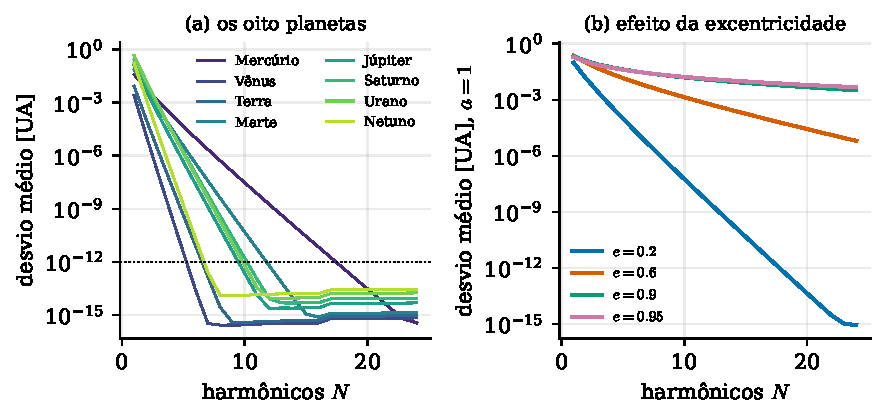
\includegraphics[width=\textwidth]{convergencia.pdf}
  \legend{(a) Os oito planetas; a linha pontilhada é o piso de $10^{-12}$\,UA. (b) Órbitas hipotéticas com $a = 1$\,UA: quanto mais alongada, mais devagar a série converge. Fonte: elaborada pelos autores.}
\end{figure}

Em termos absolutos os desvios com poucos termos são grandes: milhões de quilômetros para os planetas externos com $|n|\leq1$. Em termos relativos, porém, com $|n|\leq1$ o desvio de Júpiter já é de 2,4\,\% do semieixo, e com $|n|\leq2$ todos os planetas, exceto Mercúrio, ficam abaixo de 0,4\,\% (Júpiter, 0,09\,\%). É o que \citeonline{farias2016} observou nos gráficos: dois ou três termos já são uma excelente aproximação, com a exceção de Mercúrio.

\subsubsection{Conferência da forma fechada}

Os coeficientes calculados numericamente pela \autoref{eq:dft} foram comparados com a forma fechada da \autoref{eq:cn-bessel}. Para Mercúrio, com $|n|\leq 24$, a maior diferença foi de $2\times10^{-16}$\,UA, o arredondamento da aritmética de dupla precisão. Para órbitas hipotéticas com $a = 1$\,UA, a diferença foi de $4\times10^{-16}$ em $e = 0{,}6$, $1{,}2\times10^{-14}$ em $e = 0{,}9$ e $1{,}4\times10^{-8}$ em $e=0{,}95$. Neste último caso o aliasing descrito na \autoref{sec:dft} já aparece: o espectro decai devagar demais para 720 amostras. A relação $c_0 = -\frac32 ae$ (\autoref{eq:c0}) se verificou com erro relativo de $10^{-15}$ para os oito planetas.

\subsection{Copérnico revisitado}\label{sec:copernico-revisitado}

O \autoref{sec:pequeno-e} mostrou que, até primeira ordem na excentricidade, a série de Fourier no tempo de uma órbita kepleriana tem três termos: um deslocamento fixo $c_0 = -\frac32 ae$, um deferente $c_1\approx a$ e um epiciclo $c_2\approx\frac12 ae$ que gira com o dobro da frequência (\autoref{eq:copernico-fourier}).

Considere agora o modelo do \emph{Commentariolus} (\autoref{tab:copernico-raios}). Na descrição usual do mecanismo \cite{gallavotti1999,sugon2008}, o centro do primeiro epiciclo percorre o deferente, centrado no centro da órbita da Terra (o Sol médio, deslocado do Sol), enquanto o raio do epiciclo gira em sentido contrário com o mesmo período, de modo que, \emph{visto de fora}, ele mantém orientação fixa. O segundo epiciclo, montado na ponta do primeiro, gira duas vezes por período. Escrevendo cada movimento como número complexo, com a anomalia média $M$ medida a partir do periélio,
\begin{equation}
  z_\text{Copérnico}(M) = -r_1 + R\,e^{\ii M} + r_2\,e^{2\ii M}.
  \label{eq:copernico-modelo} % PENDENTE-E5: efeito do Sol médio em c0 (Tarefa 10)
\end{equation}
É a \autoref{eq:copernico-fourier} com $R \leftrightarrow a$, $r_1 \leftrightarrow \frac32 ae$ e $r_2 \leftrightarrow \frac12 ae$. Em particular, o modelo de Copérnico tem $r_1/r_2 = 3$ para \emph{todos} os planetas, e essa é exatamente a razão $\frac32 : \frac12$ que a série de Fourier impõe. A \autoref{tab:copernico-fourier} e a \autoref{fig:copernico} comparam os números.

\begin{table}[htb]
  \centering
  \caption{Raios de Copérnico comparados com os coeficientes de Fourier da órbita moderna}
  \label{tab:copernico-fourier}
  \small
  \setlength{\tabcolsep}{4.5pt}
  \begin{tabular}{l cc cc cc cc}
    \toprule
    & \multicolumn{2}{c}{Deferente} & \multicolumn{2}{c}{Excêntrico} & \multicolumn{2}{c}{Epiciclo duplo} & \multicolumn{2}{c}{Excentricidade} \\
    \cmidrule(lr){2-3}\cmidrule(lr){4-5}\cmidrule(lr){6-7}\cmidrule(lr){8-9}
    Planeta & $R$ & $a$ & $r_1$ & $|c_0|$ & $r_2$ & $|c_2|$ & $\frac{r_1}{1{,}5R}$ & $e$ \\
    \midrule
    Mercúrio & 0,376 & 0,387 & 0,067 & 0,119 & 0,023 & 0,039 & 0,119 & 0,206 \\
    Vênus    & 0,720 & 0,723 & 0,030 & 0,007 & 0,010 & 0,002 & 0,028 & 0,007 \\
    Marte    & 1,520 & 1,524 & 0,223 & 0,214 & 0,074 & 0,071 & 0,098 & 0,093 \\
    Júpiter  & 5,217 & 5,202 & 0,404 & 0,377 & 0,135 & 0,125 & 0,052 & 0,048 \\
    Saturno  & 9,207 & 9,546 & 0,787 & 0,793 & 0,263 & 0,264 & 0,057 & 0,055 \\
    \bottomrule
  \end{tabular}
  \legend{Raios em unidades astronômicas, convertidos das partes de Copérnico dividindo por 25. Os coeficientes $|c_0|$ e $|c_2|$ são da órbita osculadora em 1/1/2026. Fonte: elaborada pelos autores, com os raios de Copérnico de \citeonline{farias2016}.}
\end{table}

\begin{figure}[htb]
  \centering
  \caption{Os epiciclos de Copérnico e os coeficientes de Fourier}
  \label{fig:copernico}
  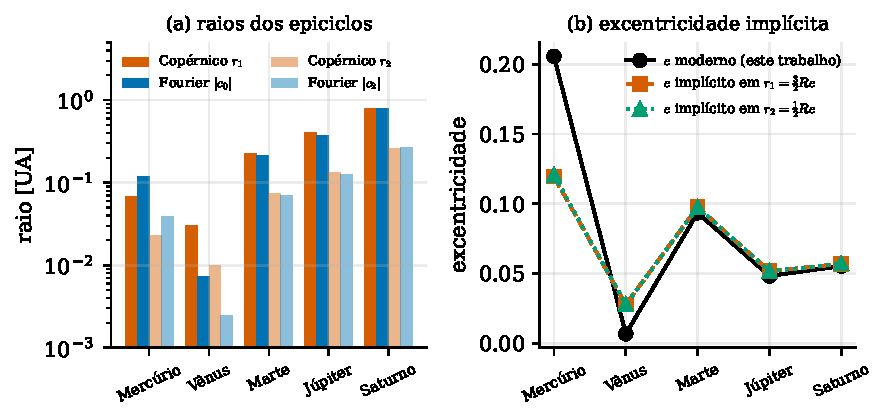
\includegraphics[width=\textwidth]{copernico.pdf}
  \legend{(a) Raios em escala logarítmica. (b) A excentricidade implícita em cada epiciclo de Copérnico, comparada com a moderna; as duas estimativas coincidem porque $r_1/r_2 = 3$. Fonte: elaborada pelos autores.}
\end{figure}

Para Marte, Júpiter e Saturno a concordância é boa. Os deferentes reproduzem os semieixos com erro de 0,2\,\% a 3,6\,\%, e os dois epiciclos reproduzem $|c_0|$ e $|c_2|$ com erro de 0,4\,\% a 8\,\%. A excentricidade implícita nos raios de Copérnico, $r_1/(1{,}5R)$, fica a menos de 0,005 da moderna nos três casos. Com a mesma métrica usada na \autoref{sec:res-fourier}, o modelo de Copérnico com os números dele erra a posição de Marte em no máximo 0,017\,UA, ou 1,1\,\% do semieixo; o de Júpiter em 0,9\,\%. Em Saturno o erro chega a 3,6\,\%, quase todo vindo do deferente, e não dos epiciclos.

Para Mercúrio e Vênus a concordância é pior, e por razões diferentes. Em Mercúrio a excentricidade é grande o bastante para que os termos de segunda ordem, desprezados na \autoref{eq:copernico-fourier}, cheguem a 10--15\,\% dos de primeira; além disso, o modelo de Mercúrio é historicamente o mais complicado da astronomia pré-kepleriana. Em Vênus a órbita é quase circular, e a excentricidade implícita (0,028) é quatro vezes a real; uma hipótese plausível, que não investigamos, é que os dados de Copérnico para Vênus carreguem a marca da excentricidade da própria órbita da Terra (0,017), da qual um planeta interior é sempre observado.

\begin{paraaprofundar}[: a relação com o TCC]
\citeonline{farias2016} comparou os raios de Copérnico com os raios da série de Fourier das órbitas reais e concluiu que eles têm a mesma ordem de grandeza, especialmente o primeiro epiciclo. Nas simulações daquele trabalho, o primeiro epiciclo foi modelado girando com frequência $-\omega$ e o segundo com $2\omega$, e uma modificação para as frequências $\omega$, $2\omega$ e $3\omega$ melhorou o ajuste. A leitura adotada aqui atribui ao primeiro epiciclo frequência \emph{zero} no referencial fixo, o que transforma o primeiro epiciclo no excêntrico $c_0$. Com essa atribuição, a comparação passa a ser termo a termo e a concordância passa de ordem de grandeza para poucos por cento. Com a mesma métrica, o modelo com frequências $(1, -1, 2)$ erra a posição de Marte em até 0,44\,UA, contra 0,017\,UA da leitura com frequência zero. O resultado não seria possível sem a organização dos dados históricos feita naquele trabalho. A conclusão de \citeonline{farias2016} de que um modelo ``heliostático'', com o Sol fora do centro do deferente, seria mais preciso é, nessa leitura, exatamente o que Copérnico fez: o excêntrico $r_1$ é o deslocamento entre o Sol e o centro efetivo do movimento.
\end{paraaprofundar}

Em primeira ordem na excentricidade, portanto, os raios do modelo de Copérnico para Marte, Júpiter e Saturno reproduzem os coeficientes da série de Fourier da órbita kepleriana, e a razão entre os dois epiciclos é a da série. Não comparamos esse resultado com outros modelos da mesma ordem, como o de Ptolomeu com equante. Sem essa comparação, os números mostram que os raios de Copérnico estavam bem estimados, mas não que o modelo dele seja o único a reproduzir a série.

\subsection{Solução da equação de Kepler}

A \autoref{fig:kepler-iteracoes} mede o número de iterações de Newton necessário para resolver a \autoref{eq:kepler} com tolerância de $10^{-13}$, no pior valor de $M$, para cada excentricidade. Com o chute $E_0 = M$, a convergência é rápida até $e\approx 0{,}98$, mas a partir daí há valores de $M$, perto do periélio, em que o método oscila e não converge. Com o chute de Danby, nunca são necessárias mais de 12 iterações, mesmo em $e = 0{,}999$. Os planetas, com $e < 0{,}21$, nunca precisam de mais de 5. O teste mostra também que o limite de 0,8 citado num comentário do código para a falha do chute $E_0=M$ é conservador; o limite medido é perto de 0,99.

\begin{figure}[htb]
  \centering
  \caption{Iterações de Newton para resolver a equação de Kepler}
  \label{fig:kepler-iteracoes}
  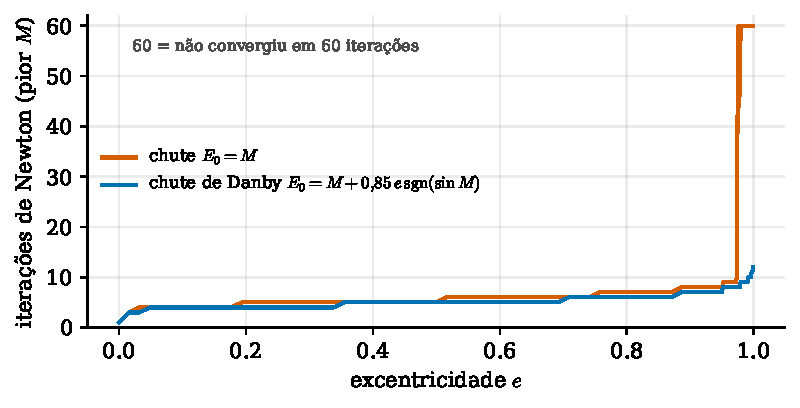
\includegraphics[width=0.85\textwidth]{kepler_iteracoes.pdf}
  \legend{Pior caso sobre $M\in(0,2\pi)$, com amostragem refinada perto de $M = 0$. Fonte: elaborada pelos autores.}
\end{figure}

\subsection{Erro das luas}\label{sec:res-luas}

A \autoref{tab:luas} mostra o erro de posição das treze luas propagadas analiticamente, medido contra o JPL Horizons entre 2020 e 2040, a cada 13 dias. Os parâmetros foram ajustados em dados de 2000 a 2016, de modo que essa janela mede o erro do \emph{modelo} e não o do ajuste. O erro não cresce de forma sistemática: a razão entre o pior erro da segunda e o da primeira metade da janela fica entre 0,97 e 1,07 para seis das treze luas e não passa de 1,7 em nenhuma. Ele vem de termos periódicos, como as ressonâncias entre as galileanas, que um modelo de dois corpos com precessão não contém.

\begin{table}[htb]
  \centering
  \caption{Erro das luas contra o JPL Horizons, 2020--2040}
  \label{tab:luas}
  \small
  \begin{tabular}{llrrrr}
    \toprule
    Lua & Planeta & $a$ (km) & Erro máximo (km) & Erro RMS (km) & Máximo / $a$ \\
    \midrule
    Lua      & Terra   & 384\,400   & 15\,293 & 7\,655  & 4,0\,\% \\
    Fobos    & Marte   & 9\,375     & 822     & 375     & 8,8\,\% \\
    Deimos   & Marte   & 23\,457    & 456     & 279     & 1,9\,\% \\
    Io       & Júpiter & 421\,800   & 7\,699  & 3\,943  & 1,8\,\% \\
    Europa   & Júpiter & 671\,100   & 25\,702 & 13\,725 & 3,8\,\% \\
    Ganimedes& Júpiter & 1\,070\,400 & 4\,295 & 2\,265  & 0,4\,\% \\
    Calisto  & Júpiter & 1\,882\,700 & 3\,587 & 2\,546  & 0,2\,\% \\
    Encélado & Saturno & 238\,400   & 5\,710  & 2\,679  & 2,4\,\% \\
    Titã     & Saturno & 1\,221\,900 & 37\,329 & 21\,211 & 3,1\,\% \\
    Titânia  & Urano   & 436\,298   & 2\,088  & 977     & 0,5\,\% \\
    Oberon   & Urano   & 583\,511   & 2\,476  & 1\,372  & 0,4\,\% \\
    Miranda  & Urano   & 129\,846   & 9\,423  & 5\,789  & 7,3\,\% \\
    Tritão   & Netuno  & 354\,800   & 52\,636 & 29\,194 & 14,8\,\% \\
    \bottomrule
  \end{tabular}
  \legend{Fonte: arquivo \arquivo{derivaDasLuas.json}, gerado por \arquivo{ferramentas/conferir\_luas.mjs}.}
\end{table}

\subsection{Fenômenos que emergem da simulação}

Nada no código manda o Sol se mover nem Marte recuar no céu. Os dois movimentos resultam da integração, o que os torna bons exemplos para a sala de aula.

O primeiro é o movimento retrógrado de Marte, já mostrado na \autoref{fig:marte-retrogrado}: o programa prevê a retrogradação de 2027 entre 10 de janeiro e 1º de abril. O segundo é o movimento do Sol em torno do centro de massa do sistema (\autoref{fig:sol-baricentro}). Em cinquenta anos, o centro do Sol percorre um emaranhado de laços que chega a 1,8 raio solar do baricentro: o centro de massa do Sistema Solar fica, boa parte do tempo, \emph{fora} do Sol. O padrão é dominado por Júpiter, com período de 12 anos, modulado por Saturno. É esse movimento que, medido em outras estrelas pelo efeito Doppler, revela a existência de planetas extrassolares.

\begin{figure}[htb]
  \centering
  \caption{O centro do Sol em torno do centro de massa do sistema, 2026--2076}
  \label{fig:sol-baricentro}
  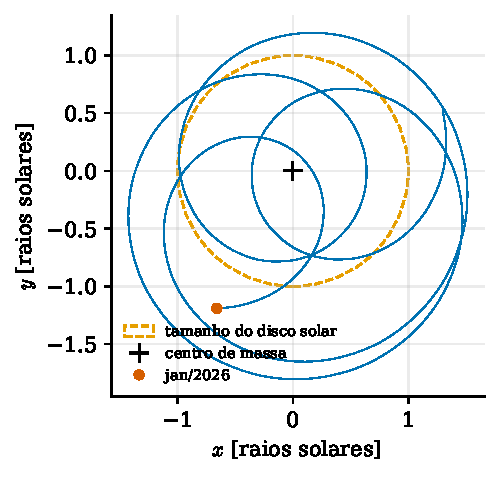
\includegraphics[width=0.55\textwidth]{sol_baricentro.pdf}
  \legend{Projeção no plano da eclíptica. O círculo tracejado tem o raio do Sol. Fonte: elaborada pelos autores com o integrador do programa.}
\end{figure}
